%        1         2         3         4         5         6         7         8         9         0         1         2
%23456789012345678901234567890123456789012345678901234567890123456789012345678901234567890123456789012345678901234567890
\documentclass[12pt]{MIA-USA}

\usepackage{layout}
\usepackage{subcaption}
\usepackage{paralist}
\usepackage{breakcites}

\usepackage[pagebackref=true,breaklinks=true]{hyperref}
\hypersetup{
	pdftitle={Documento de trabajo Final Maestría Inteligencia Artificial}, 
	pdfauthor={MIA-D.Martinez}, 
	pdfsubject={}, 
	pdfcreator={DarMart with Latex}, 
	colorlinks=true,
	linkcolor=GrisUno,
	citecolor=AzulInstitucional,
	filecolor=AzulClaro,
	urlcolor=AzulInstitucional,
	linktoc=all
}

\graphicspath{{Images/}}


\title{T\'itulo del proyecto}
\author{Nombres y apellidos Estudiante}
\documenttype{Docuemnto Final de Maestr\'ia}

\advisor{Nombres y apellidos Asesor}

% Si hay un coasesor 
% \coadvisor{Nombres y apellidos Co-Asesor}


% Aqui comienza el documento
% - -- --- ----- ------- ------- ----- --- -- -
\begin{document}
    % \layout{}
	
	\maketitle
	% Incluye la pagina de acptación (Opcional)
	\input{FrontMatter/F01-Approval}
	% Incluye la dedicatoria (Opcional)
	%  Nota mediante la cual el autor ofrece su trabajo, en forma especial, a personas o entidades. Su presentación es opcional y debe conservar los márgenes
\subsection*{Dedicatoria}
\vspace*{1.5cm}
{\hfill
    \begin{minipage}{0.5\textwidth}
        \noindent
         Nota mediante la cual el autor ofrece su trabajo, en forma especial, a personas o entidades~\cite{NTC14862008}. Su presentación es opcional y, aunque cada autor podr\'{a} determinar la distribuci\'{o}n del texto en la p\'{a}gina, se sugiere esta presentaci\'{o}n. En ella el autor dedica su trabajo en forma especial a personas y/o entidades.\\
         \vspace*{0.5cm}
         
         Por ejemplo:\\
         \\
         A mis padres\\
         \vspace*{1.0cm}
         
         o\\
         \vspace*{1.0cm}
         
        A computer would deserve to be called intelligent if it could deceive a human into believing that it was human.\\\\
        Alan Turing\\
    
    \end{minipage}
}
\newpage
	% Incluye los agradecimientos (Opcional)
	% Página de agradecimientos. En ella el (los) autor (es) expresa (n) el reconocimiento hacia las personas y entidades que asesoraron técnicamente, suministraron datos, financiaron total o parcialmente la investigación o contribuyeron significativamente al desarrollo del tema. Es opcional y debe contener, además de la nota correspondiente, los nombres de las personas con sus respectivos cargos y los nombres completos de las instituciones y su aporte al trabajo.

\section*{Agradecimientos}

Página de agradecimientos. En ella el (los) autor (es) expresa (n) el reconocimiento hacia las personas y entidades que asesoraron técnicamente, suministraron datos, financiaron total o parcialmente la investigación o contribuyeron significativamente al desarrollo del tema. Es opcional y debe contener, además de la nota correspondiente, los nombres de las personas con sus respectivos cargos y los nombres completos de las instituciones y su aporte al trabajo~\cite{NTC14862008}.


%  Se debe dejar la nueva página para guardar el orden de las seciones
\newpage
	% Resumen
 	% Presentación abreviada y precisa del contenido de un documento, sin agregar interpretación o crítica y se recomienda un exceda una página.
\section*{Resumen}


El resumen es una presentación abreviada y precisa del contenido de un documento, sin agregar interpretación o crítica. Para documentos extensos como informes, tesis y trabajos de grado, no debe exceder de 500 palabras, y debe ser lo suficientemente breve para que no ocupe más de una página~\cite{NTC14862008}. Se recomienda que este resumen sea anal\'{\i}tico, es decir, que sea completo, con informaci\'{o}n cuantitativa y cualitativa, generalmente incluyendo los siguientes aspectos: objetivos, dise\~{n}o, lugar y circunstancias, pacientes (u objetivo del estudio), intervenci\'{o}n, mediciones y principales resultados, y conclusiones. Al final del resumen se deben usar palabras claves tomadas del texto (m\'{\i}nimo 3 y m\'{a}ximo 10 palabras), las cuales permiten la recuperaci\'{o}n de la informaci\'{o}n.\\

\textbf{\small Palabras clave: (m\'{a}ximo 10 palabras, preferiblemente seleccionadas de las listas internacionales que permitan el indizado cruzado)}.\\

% debe incluir una lista de palabras clave 
\textbf{Palabras clave}: palabra 1, palabra 2, palabra 3, ...

% Incluir un resumen en otro idioma de preferencia inglés
\newpage
\section*{Abstract}

% debe incluir una lista de palabras clave en el otro idioma
\textbf{Keywords}: Keyword 1, Keyword 2, Keyword 3, ...


	
    
    % Crea la tabla de contenidos a partir de la estructura del documento
    \tableofcontents
    % Crea la lista de figuras (Opcional)
    \listoffigures
    % Crea la lista de tablas (Opcional)
    \listoftables
    % Incluye la lista de simbolos (Opcional)
    \input{FrontMatter/F05-Symbols}
    % Glosario (Opcional)
 	\input{FrontMatter/F06-Glossary}
    
    
    % A partir de este punto se crea la estructura del documento con un archivo por capitulo conservando la siguiente jerarquía
    % chapter (Capitulo)
    %   - section (sección)
    %       - subsection (subsección)
    %           - subsubsection (subsubsección)
    
    % Introduction
    \chapter{Introducci\'on}
    % En ella, el autor presenta y señala la importancia, el origen (los antecedentes teóricos y prácticos), los objetivos, los alcances, las limitaciones, la metodología empleada, el significado que el estudio tiene en el avance del campo respectivo y su aplicación en el área investigada.

De acuerdo con la NTC1486, la introducción es un espacio dónde el autor presenta y señala la importancia, el origen (los antecedentes teóricos y prácticos), los objetivos, los alcances, las limitaciones, la metodología empleada, el significado que el estudio tiene en el avance del campo respectivo y su aplicación en el área investigada. No debe confundirse con el resumen, ni contener un recuento detallado de la teoría, el método o los resultados, como tampoco anticipar las conclusiones y recomendaciones~\cite{NTC14862008}, y se recomienda que la introducci\'{o}n tenga una extensi\'{o}n de m\'{\i}nimo 2 p\'{a}ginas y m\'{a}ximo de 4 p\'{a}ginas.\\

Para el desarrollo del documento utilizando la plantilla en \LaTeX se recomienda la guía \textit{the not so short guide to \LaTeX}~\cite{Oetiker2016} que brinda una introducci\'on breve pero muy completa. En donde se presentan entro otras cosas los comandos y ambeintes para el trabajo con gr\'aficas y tablas, como las que se muestran a continuaci\'on:

\begin{figure}[htbp!]
    \caption{Muestra de inclusio\'on de un elemento gr\'afico}
    \centering
    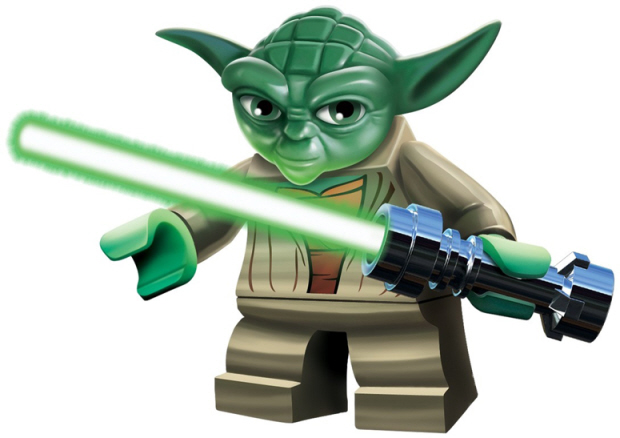
\includegraphics[width=0.8\textwidth]{Images/ImagenYoda.jpg}
    \label{fig:yoda}
\end{figure}

As\'i la Figura~\ref{fig:yoda} muestra una imagen que se encuentra en el directorio images, mientras la tabla~\ref{tab:tablasEx}, muestra dos ejemplos de información tabular con combinaci\'on de columnas, y combinaci\'on de filas.

\begin{table}[htbp!]
    \centering
    \caption{Ejemplo de tabla con multi columnas (arriba) y multi filas(abajo)}
    \begin{tabular}{ |p{3cm}||p{3cm}|p{3cm}|p{3cm}|  }
        \hline
        \multicolumn{4}{|c|}{Country List} \\
        \hline
        Country Name or Area Name& ISO ALPHA 2 Code &ISO ALPHA 3 Code&ISO numeric Code\\
        \hline
        Afghanistan   & AF    &AFG&   004\\
        Aland Islands&   AX  & ALA   &248\\
        Albania &AL & ALB&  008\\
        Algeria    &DZ & DZA&  012\\
        American Samoa&   AS  & ASM&016\\
        Andorra& AD  & AND   &020\\
        Angola& AO  & AGO&024\\
        \hline
    \end{tabular}\\
    \vspace{0.5cm}
    \begin{tabular}{ |c|c|c|c| } 
        \hline
        col1 & col2 & col3 \\
        \hline
        \multirow{3}{4em}{Multiple row} & cell2 & cell3 \\ 
        & cell5 & cell6 \\ 
        & cell8 & cell9 \\ 
        \hline
    \end{tabular}

    \label{tab:tablasEx}
\end{table}

Adem\'as se recomienda consultar los manuales que aparecen en al secci\'on de aprendizaje de overleaf, por ejemplo el de \href{https://www.overleaf.com/learn/latex/Tables}{tablas}.

La presente plantilla tiene en cuenta aspectos importantes de la Norma T\'{e}cnica Colombiana - NTC 1486~\cite{NTC14862008}. Las m\'{a}rgenes, numeraci\'{o}n, tama\~{n}o de las fuentes y dem\'{a}s aspectos de formato, deben ser conservada de acuerdo con esta plantilla, la cual esta dise\~{n}ada para imprimir por lado y lado en hojas tama\~{n}o carta. Se sugiere que los encabezados cambien seg\'{u}n la secci\'{o}n/cap\'{i}tulo del documento.\\

La redacci\'{o}n debe ser impersonal y gen\'{e}rica. La numeraci\'{o}n de las hojas sugiere que las p\'{a}ginas preliminares se realicen en n\'{u}meros romanos en may\'{u}scula y las dem\'{a}s en n\'{u}meros ar\'{a}bigos, en forma consecutiva a partir de la introducci\'{o}n que comenzar\'{a} con el n\'{u}mero 1. La cubierta y la portada no se numeran pero si se cuentan como p\'{a}ginas.\\

Para trabajos muy extensos se recomienda publicar m\'{a}s de un volumen. Se debe tener en cuenta que algunas facultades tienen reglamentada la extensi\'{o}n m\'{a}xima de las tesis  o trabajo de investigaci\'{o}n; en caso que no sea as\'{\i}, se sugiere que el documento no supere 120 p\'{a}ginas.\\

No se debe utilizar numeraci\'{o}n compuesta como 13A, 14B \'{o} 17 bis, entre otros, que indican superposici\'{o}n de texto en el documento. Para resaltar, puede usarse letra cursiva o negrilla. Los t\'{e}rminos de otras lenguas que aparezcan dentro del texto se escriben en cursiva.\\

El contenido de este documento esta basado principalmente en la NTC1486~\cite{NTC14862008} y la plantilla de Tesis de maestr\'ia y doctorado de la Universidad Nacional de colombia~\cite{Unal2014DocTesis}.

    
    % Capitulo 2
    \chapter{Cap\'{i}tulo 1}
    \input{MainMatter/Cap1/M02-Chapter1}
    
    % Capitulo 2 - Estado del arte
    \chapter{Estado del arte}
    % Estado del arte: simuladores de redes existentes, con énfasis en las
% herramientas aplicables a redes descentralizadas (ad-hoc/mesh, P2P y
% de consenso distribuido).

La evaluación de un protocolo de red rara vez se hace desplegando la red
completa: el costo, la dificultad de reproducir las condiciones del canal y la
imposibilidad de repetir un experimento con exactitud han hecho de la
simulación la herramienta dominante en el área. Este capítulo revisa las
herramientas de simulación de redes disponibles hoy, distingue las que
permiten estudiar redes descentralizadas de las de propósito general y, a
partir de esa revisión, delimita el vacío que el presente trabajo pretende
cubrir.

\section{Simuladores de redes de propósito general}
\label{sec:simuladores-generales}

La primera generación de herramientas ampliamente adoptadas por la comunidad
académica se organiza alrededor del paradigma de \textit{simulación por
eventos discretos}: el estado de la red avanza saltando de un evento
(transmisión, recepción, expiración de un temporizador) al siguiente, sin
recorrer el tiempo de forma continua.

\textbf{ns-2 y ns-3.} El simulador ns-2, desarrollado en el marco del proyecto
VINT, fue durante casi dos décadas la referencia de facto en investigación de
redes~\cite{Ns2VintProject}. Su sucesor, ns-3, reescribió el núcleo
completamente en C++ e incorporó una pila TCP/IP completa junto con modelos de
tecnologías inalámbricas como IEEE 802.11, LTE y WiMAX~\cite{Riley2010ns3}. La
posibilidad de integrar ns-3 con bancos de pruebas y aplicaciones reales lo
convirtió en el estándar aceptado por la comunidad para publicar resultados.

\textbf{OMNeT++ e INET.} OMNeT++ es un entorno modular de simulación por
eventos discretos escrito en C++, concebido como una infraestructura genérica
más que como un simulador de redes cerrado~\cite{Varga2008Omnetpp}. La
funcionalidad de red propiamente dicha la aporta el marco de trabajo INET, una
biblioteca de modelos que incluye la pila de Internet, protocolos de enlace
cableados e inalámbricos, modelos de movilidad y un conjunto de protocolos de
enrutamiento para redes ad-hoc.

\textbf{GloMoSim y QualNet.} GloMoSim se propuso específicamente para la
simulación paralela de redes inalámbricas de gran escala, organizando la pila
de comunicaciones en capas con una API propia por capa, de modo que los
modelos de una capa interactúan con los de la capa adyacente únicamente a
través de esas interfaces~\cite{Zeng1998Glomosim}. Su evolución comercial,
QualNet, y otras herramientas propietarias como Riverbed Modeler (antes
OPNET) y NetSim, ocupan el mismo nicho con soporte comercial y bibliotecas de
modelos más extensas.

El rasgo que comparten todas estas herramientas, y que resulta central para
este trabajo, es que \textbf{el protocolo bajo estudio se reimplementa como un
modelo dentro del simulador}. Lo que se valida experimentalmente es, en
sentido estricto, ese modelo, no la implementación que después se despliega en
un dispositivo real.

\section{Herramientas orientadas a redes descentralizadas}
\label{sec:simuladores-descentralizados}

El término \textit{red descentralizada} se emplea en la literatura con al
menos tres alcances distintos, y a cada uno le corresponde una familia
diferente de herramientas. Conviene separarlas antes de compararlas.

\subsection{Redes ad-hoc móviles y redes malladas}
\label{subsec:manet}

Son redes sin infraestructura fija, en las que cada nodo actúa
simultáneamente como terminal y como encaminador. Las herramientas
disponibles se reparten entre simuladores y emuladores:

\begin{itemize}
\item \textbf{ns-3} incluye modelos de los protocolos de enrutamiento ad-hoc
clásicos (AODV, OLSR, DSDV y DSR) sobre su modelo de canal
inalámbrico~\cite{Riley2010ns3}.

\item \textbf{INET sobre OMNeT++} ofrece un conjunto equivalente de protocolos
MANET junto con modelos de movilidad configurables~\cite{Varga2008Omnetpp}.

\item \textbf{Cooja}, el simulador del sistema operativo Contiki para redes de
sensores, introduce la noción de \textit{simulación multinivel}: permite
simular simultáneamente a nivel de red, de sistema operativo y de instrucción
de máquina, ejecutando el firmware real del nodo sobre una emulación del
hardware~\cite{Osterlind2006Cooja}. TOSSIM, del ecosistema TinyOS, sigue una
estrategia comparable.

\item \textbf{EMANE} (\textit{Extendable Mobile Ad-hoc Network Emulator})
aporta modelos de radio y de capa física detallados, pensados expresamente
para emular redes MANET, y suele integrarse con otros
emuladores~\cite{Nrl2023Emane}.

\item \textbf{CORE} (\textit{Common Open Research Emulator}) es un emulador en
tiempo real que instancia topologías híbridas compuestas por nodos virtuales y
hardware real, apoyándose en la virtualización de la pila de red del sistema
operativo; escala a topologías de más de un centenar de nodos virtuales sobre
un único servidor~\cite{Ahrenholz2008Core}.

\item \textbf{Mininet-WiFi} extiende Mininet a redes inalámbricas definidas por
software: cada nodo es un proceso ubicado en un espacio de nombres de red de
Linux, interconectado mediante pares de interfaces virtuales, de manera que
cualquier programa que corra sobre Linux corre sin modificaciones dentro de la
topología emulada~\cite{Fontes2015MininetWifi}.
\end{itemize}

\subsection{Redes entre pares y superposiciones descentralizadas}
\label{subsec:p2p}

Cuando la descentralización ocurre en la capa de aplicación y no en la capa
física, el objeto de estudio deja de ser el canal inalámbrico y pasa a ser la
topología lógica de la superposición (\textit{overlay}). Las herramientas
representativas son:

\begin{itemize}
\item \textbf{PeerSim}, diseñado para escalar hasta del orden de un millón de
nodos, a costa de un modelo deliberadamente abstracto que prescinde por
completo de las capas inferiores~\cite{Montresor2009Peersim}.

\item \textbf{OverSim}, construido sobre OMNeT++, que combina modelos de
superposiciones estructuradas y no estructuradas (Chord, Pastry, Kademlia) con
la posibilidad de ejecutar aplicaciones de red reales sobre el mismo
código~\cite{Baumgart2009Oversim}.

\item \textbf{PlanetSim} y \textbf{PeerfactSim.KOM}, orientados a la evaluación
comparativa sistemática de sistemas entre pares.
\end{itemize}

\subsection{Redes descentralizadas con consenso distribuido}
\label{subsec:blockchain}

Una tercera lectura de \textit{descentralizado} corresponde a los sistemas de
registro distribuido. \textbf{SimBlock} es un simulador de red de cadena de
bloques dirigido por eventos que permite modificar con facilidad el
comportamiento de los nodos, de modo que puede estudiarse cómo influye ese
comportamiento sobre la red en su conjunto~\cite{Aoki2019Simblock}.
\textbf{BlockSim}, escrito en Python sobre la biblioteca SimPy, cubre un
propósito similar para Ethereum y Bitcoin. Estas herramientas modelan la
propagación de bloques y el consenso, pero no la capa física ni la movilidad,
por lo que quedan fuera del alcance de este trabajo.

\section{Simulación, emulación y ejecución de código real}
\label{sec:simulacion-vs-emulacion}

La revisión anterior muestra que las herramientas no se distinguen solamente
por el dominio que cubren, sino por un eje más determinante: qué tan cerca
está el código evaluado del código que finalmente se despliega. Pueden
distinguirse tres niveles:

\begin{itemize}
\item \textbf{Simulación pura.} El protocolo se reimplementa como modelo dentro
del simulador. Escala bien y es perfectamente reproducible, pero introduce una
brecha entre el modelo validado y la implementación desplegada.

\item \textbf{Emulación.} El código real se ejecuta sobre un sistema operativo
virtualizado o sobre espacios de nombres de red. La fidelidad es alta, pero
cada nodo cuesta recursos del sistema anfitrión y el modelado del medio radio
requiere componentes adicionales o hardware específico.

\item \textbf{Enfoques híbridos o multinivel.} El código real del protocolo se
ejecuta sobre un modelo del medio, como en la simulación multinivel de
Cooja~\cite{Osterlind2006Cooja}.
\end{itemize}

La Tabla~\ref{tab:comparativa-simuladores} resume las herramientas revisadas
según estos criterios.

\begin{table}[htbp!]
    \centering
    \caption{Comparación de las herramientas de simulación y emulación revisadas}
    \label{tab:comparativa-simuladores}
    \footnotesize
    \begin{tabular}{|p{2.6cm}|p{2.0cm}|p{3.4cm}|p{3.6cm}|}
        \hline
        \textbf{Herramienta} & \textbf{Tipo} & \textbf{Dominio principal} & \textbf{Código del protocolo} \\
        \hline
        ns-3 & Simulador & Redes en general, MANET & Modelo reimplementado \\
        \hline
        OMNeT++ / INET & Simulador & Redes en general, MANET & Modelo reimplementado \\
        \hline
        GloMoSim / QualNet & Simulador & Redes inalámbricas a gran escala & Modelo reimplementado \\
        \hline
        Cooja & Multinivel & Redes de sensores (Contiki) & Firmware real sobre hardware emulado \\
        \hline
        EMANE & Emulador & MANET, capa física detallada & Código real del sistema \\
        \hline
        CORE & Emulador & Topologías híbridas en tiempo real & Código real del sistema \\
        \hline
        Mininet-WiFi & Emulador & Redes inalámbricas definidas por software & Binarios reales de Linux \\
        \hline
        PeerSim & Simulador & Superposiciones entre pares & Modelo abstracto \\
        \hline
        OverSim & Simulador & Superposiciones estructuradas & Modelo y aplicaciones reales \\
        \hline
        SimBlock & Simulador & Redes de cadena de bloques & Modelo de propagación \\
        \hline
    \end{tabular}
\end{table}

\section{El protocolo B.A.T.M.A.N. en la literatura}
\label{sec:batman-literatura}

B.A.T.M.A.N. (\textit{Better Approach To Mobile Ad-hoc Networking}) fue
propuesto como alternativa a los protocolos de estado de enlace para redes
malladas comunitarias, y se encuentra especificado como borrador de la
IETF~\cite{Neumann2008Batman}. A diferencia de OLSR, ningún nodo construye una
visión completa de la topología: cada nodo conoce únicamente cuál de sus
vecinos es el mejor siguiente salto hacia cada destino, decisión que toma a
partir de la calidad de transmisión (TQ) acumulada de los mensajes de
originador (OGM) que recibe. Esta decisión de diseño reduce la sobrecarga de
señalización y la sensibilidad a la información topológica desactualizada.

Su implementación de referencia, \textit{batman-adv}, opera en la capa de
enlace y está incorporada al núcleo de Linux, lo que la convierte en una de
las pocas implementaciones de protocolos de enrutamiento ad-hoc con despliegue
real sostenido en redes comunitarias~\cite{OpenMesh2024Batmanadv}. En cuanto
a su evaluación, la literatura reporta estudios de desempeño frente a enlaces
asimétricos y trabajos de modelado y verificación formal del protocolo. Es
significativo que estas evaluaciones se apoyen mayoritariamente en modelos del
protocolo construidos dentro de un simulador, y no en la implementación
efectivamente desplegada.

\section{Redes ad-hoc en escenarios de emergencia}
\label{sec:redes-desastre}

El escenario de aplicación que motiva este trabajo cuenta con una línea de
investigación propia. Las redes ad-hoc multisalto han sido estudiadas de forma
sistemática como respuesta al problema de las comunicaciones en zonas de
desastre, donde la infraestructura fija resulta destruida o
saturada~\cite{Reina2015Disaster}. Las propiedades que las hacen adecuadas en
ese contexto son el despliegue rápido, la configuración mínima, la
conectividad multisalto y la capacidad de auto-reparación ante la pérdida de
nodos. Los trabajos revisados en esa línea coinciden en señalar la evaluación
de protocolos de enrutamiento y de esquemas de difusión como uno de los
frentes abiertos.

\section{Brecha identificada}
\label{sec:brecha}

De la revisión anterior se desprenden tres observaciones que, en conjunto,
delimitan el aporte de este trabajo:

\begin{enumerate}
\item Los simuladores de propósito general y los orientados a MANET
(Sección~\ref{sec:simuladores-generales}) evalúan un modelo del protocolo, no
su implementación. Las conclusiones obtenidas sobre B.A.T.M.A.N. en esas
herramientas son, por tanto, conclusiones sobre el modelo.

\item Los emuladores (Sección~\ref{subsec:manet}) sí ejecutan código real, pero
al precio de un costo por nodo considerable en el anfitrión y sin un modelo de
propagación tridimensional listo para usar que dé cuenta de la atenuación
entre pisos de una edificación, que es precisamente la condición del escenario
de interés.

\item Las herramientas de redes descentralizadas de las
Secciones~\ref{subsec:p2p} y~\ref{subsec:blockchain} operan en la capa de
aplicación y no modelan ni el medio radio ni la movilidad física de los nodos.
\end{enumerate}

Existe entonces un punto intermedio poco explorado: ejecutar la
\textbf{implementación real del protocolo} —las mismas clases que correrían en
un dispositivo desplegado— dentro de un mismo proceso, sustituyendo únicamente
la capa de transporte por un modelo del medio radio que sí contemple la
geometría del edificio y la atenuación entre pisos. Esta estrategia conserva
la fidelidad del código evaluado sin incurrir en el costo por nodo de la
emulación, y es la que adopta el simulador desarrollado en este trabajo.

    
    % Capitulo 3
    \chapter{Cap\'{i}tulo 3}
    \input{MainMatter/Cap3/M04-Chapter3}
    
    % Capitulo 4
    \chapter{Cap\'{i}tulo 4}
    \input{MainMatter/Cap4/M05-Chapter4}
    
    % Capitulo 5
    \chapter{Cap\'{i}tulo 5}
    \input{MainMatter/Cap5/M06-Chapter5}
    
    % Capitulo 10
    \chapter{Conclusiones y recomendaciones}
    \input{MainMatter/Cap9/M10-Conclusiones}
    
    
    % Anexos (Opcional)
    % \chapter*{Anexos}
    % \input{BackMatter/B01-Anexos}
    
    % Indices (Opcional)
    % \chapter*{\'Indices}
    % \input{BackMatter/B10-Index}
    
	% Incluye las referencias
    \bibliographystyle{apalike}
 	\bibliography{Bibliography/referencias}

\end{document}
